\documentclass[a4paper]{article}
% generated by Docutils <http://docutils.sourceforge.net/>
\usepackage{fixltx2e} % LaTeX patches, \textsubscript
\usepackage{cmap} % fix search and cut-and-paste in Acrobat
\usepackage{ifthen}
\usepackage[T1]{fontenc}
\usepackage[utf8]{inputenc}
\usepackage{graphicx}
\setcounter{secnumdepth}{0}
\usepackage{longtable,ltcaption,array}
\setlength{\extrarowheight}{2pt}
\newlength{\DUtablewidth} % internal use in tables
\usepackage{tabularx}

%%% Custom LaTeX preamble
% PDF Standard Fonts
\usepackage{mathptmx} % Times
\usepackage[scaled=.90]{helvet}
\usepackage{courier}

%%% User specified packages and stylesheets

%%% Fallback definitions for Docutils-specific commands

% providelength (provide a length variable and set default, if it is new)
\providecommand*{\DUprovidelength}[2]{
  \ifthenelse{\isundefined{#1}}{\newlength{#1}\setlength{#1}{#2}}{}
}

% admonition (specially marked topic)
\providecommand{\DUadmonition}[2][class-arg]{%
  % try \DUadmonition#1{#2}:
  \ifcsname DUadmonition#1\endcsname%
    \csname DUadmonition#1\endcsname{#2}%
  \else
    \begin{center}
      \fbox{\parbox{0.9\linewidth}{#2}}
    \end{center}
  \fi
}

% docinfo (width of docinfo table)
\DUprovidelength{\DUdocinfowidth}{0.9\linewidth}

% title for topics, admonitions, unsupported section levels, and sidebar
\providecommand*{\DUtitle}[2][class-arg]{%
  % call \DUtitle#1{#2} if it exists:
  \ifcsname DUtitle#1\endcsname%
    \csname DUtitle#1\endcsname{#2}%
  \else
    \smallskip\noindent\textbf{#2}\smallskip%
  \fi
}

% titlereference role
\providecommand*{\DUroletitlereference}[1]{\textsl{#1}}

% hyperlinks:
\ifthenelse{\isundefined{\hypersetup}}{
  \usepackage[colorlinks=true,linkcolor=blue,urlcolor=blue]{hyperref}
  \usepackage{bookmark}
  \urlstyle{same} % normal text font (alternatives: tt, rm, sf)
}{}
\hypersetup{
  pdftitle={COSC2325-001 Course Syllabus},
}

%%% Title Data
\title{\phantomsection%
  COSC2325-001 Course Syllabus%
  \label{cosc2325-001-course-syllabus}%
  \label{spring2017-cosc2325-001-syllabus}}
\author{}
\date{}

%%% Body
\begin{document}
\maketitle

% Docinfo
\begin{center}
\begin{tabularx}{\DUdocinfowidth}{lX}
\textbf{Title}: &
Computer Architecture and Machine Language
\\
\textbf{Instructor}: &
Roie R. Black
\\
\textbf{Term}: &
Summer 2017 (9 week)
\\
\textbf{Synonym}: &
26111
\\
\textbf{Start Date}: &
May 30, 2017
\\
\textbf{website}: &
\url{http://www.co-pylit.org/classes/spring2017/cosc2325-001}
\\
\end{tabularx}
\end{center}


\section{Basic Course Information%
  \label{basic-course-information}%
}


\subsection{Course Description:%
  \label{course-description}%
}

The organization of computer systems is introduced using assembly language.
Topics include basic concepts of computer architecture and organization, memory
hierarchy, data types, computer arithmetic, control structures, interrupt
handling, instruction sets, performance metrics, and the mechanics of testing
and debugging computer systems. Embedded systems and device interfacing are
introduced


\subsection{Course Prerequisites:%
  \label{course-prerequisites}%
}

Two semesters of programming or department approval.

Studnts usually have passed COSC1336 and COSC1337 before taking this course.


\subsection{Required Text:%
  \label{required-text}%
}

\noindent\makebox[\linewidth][c]{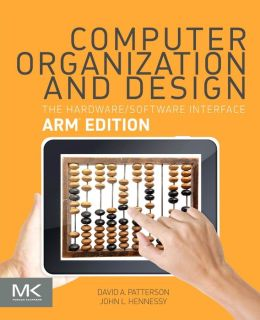
\includegraphics[width=150bp]{course/cosc2325_textbook.jpg}}

\setlength{\DUtablewidth}{\linewidth}
\begin{longtable*}[c]{|p{0.133\DUtablewidth}|p{0.365\DUtablewidth}|p{0.191\DUtablewidth}|p{0.133\DUtablewidth}|}
\hline
\textbf{%
Author(s)
} & \textbf{%
title
} & \textbf{%
ISBN
} & \textbf{%
Publisher
} \\
\hline
\endfirsthead
\hline
\textbf{%
Author(s)
} & \textbf{%
title
} & \textbf{%
ISBN
} & \textbf{%
Publisher
} \\
\hline
\endhead
\multicolumn{4}{c}{\hfill ... continued on next page} \\
\endfoot
\endlastfoot

Patterson and Hennessy
 & 
Computer Organization and Design
 & 
978-0-12-801733-3
 & 
Elsevier
 \\
\hline
\end{longtable*}


\subsection{Instructor Information%
  \label{instructor-information}%
}

\setlength{\DUtablewidth}{\linewidth}
\begin{longtable*}[c]{|p{0.191\DUtablewidth}|p{0.365\DUtablewidth}|}
\hline

Name
 & 
Roie R. Black
 \\
\hline

email
 & 
\href{mailto:rblack@austincc.edu}{rblack@austincc.edu}
 \\
\hline

Phone
 & 
512-223-3199
 \\
\hline

Office
 & 
Rio Grande - 3251 (Gym)
 \\
\hline
\end{longtable*}


\subsection{Class meetings%
  \label{class-meetings}%
}

\setlength{\DUtablewidth}{\linewidth}
\begin{longtable*}[c]{|p{0.146\DUtablewidth}|p{0.232\DUtablewidth}|p{0.232\DUtablewidth}|p{0.340\DUtablewidth}|}
\hline
\textbf{%
Event
} & \textbf{%
Day
} & \textbf{%
Time
} & \textbf{%
Room
} \\
\hline
\endfirsthead
\hline
\textbf{%
Event
} & \textbf{%
Day
} & \textbf{%
Time
} & \textbf{%
Room
} \\
\hline
\endhead
\multicolumn{4}{c}{\hfill ... continued on next page} \\
\endfoot
\endlastfoot

lecture
 & 
TTh
 & 
5:15pm - 8:15pm
 & 
HLC1-2412
 \\
\hline

Lab
 & 
MW
 & 
8:20pm - 10:00pm
 & 
HLC1-2412
 \\
\hline
\end{longtable*}


\subsection{Office Hours%
  \label{office-hours}%
}

\setlength{\DUtablewidth}{\linewidth}
\begin{longtable*}[c]{|p{0.240\DUtablewidth}|p{0.352\DUtablewidth}|p{0.352\DUtablewidth}|}
\hline
\textbf{%
Day
} & \textbf{%
Time
} & \textbf{%
Room
} \\
\hline
\endfirsthead
\hline
\textbf{%
Day
} & \textbf{%
Time
} & \textbf{%
Room
} \\
\hline
\endhead
\multicolumn{3}{c}{\hfill ... continued on next page} \\
\endfoot
\endlastfoot

TTh
 & 
3:00pm-5:00pm
 & 
HLC1-2412 or open lab
 \\
\hline

Sat
 & 
10:00am-12:00pm RGC3-3251 (by appointment only)
 &  \\
\hline
\end{longtable*}

On Saturdays, I hold RoboLab sessions where we work on course hardware, and
robot projects. I also offer help with personal system setup issues. If needed
I can be available up to 2:00pm, when the campus closes. If no one shows up
before noon, I may leave then, unless you have made an appointment.


\subsection{Instructional Methodology:%
  \label{instructional-methodology}%
}

This course will have 6 hours of lecture and 3.5 hours of lab per week. If
the students are unable to finish the assigned lab work within the lab time,
they will need to visit the CIS open labs. Teaching methodology will be to use
a hybrid approach utilizing traditional in-class lectures and lab sessions
coupled with distance-learning techniques utilizing computers and the
Internet. The students will be expected to use the lab workstations for all
homework submissions. Submission techniques will be taught during the first
few lectures. No homework will be accepted through any submission channel
except through the class lab workstations! Exams will be given in class.


\subsection{Course Rationale:%
  \label{course-rationale}%
}

This course is required as part of the Associate of Applied Science degree.


\subsection{Degree Plans:%
  \label{degree-plans}%
}
%
\begin{quote}
%
\begin{itemize}

\item This course will transfer in some form to other colleges.

\end{itemize}

\end{quote}


\subsection{Learning Outcomes/Course Objectives:%
  \label{learning-outcomes-course-objectives}%
}
%
\begin{quote}
\begin{enumerate}

\item Explain contemporary computer system organization.

\item Describe data representation in digital computers.

\item Explain the concepts of memory hierarchy, interrupt processing, and input/output mechanisms.

\item Measure the performance of a computer system.

\item Design and develop assembly language applications.

\item Explain the interfaces between software and hardware components.

\item Explain the design of instruction set architectures.

\item Develop a single - cycle processor.

\item Explain the concept of virtual memory and how it is realized in hardware and software.

\item Explain the concepts of operating system virtualization
\end{enumerate}

\end{quote}

\DUadmonition[note]{
\DUtitle[note]{Note}

In this course, we will also explore tools all modern developers should be
able to use. Specifically, we will use \DUroletitlereference{virtual machines} and \DUroletitlereference{source code
control systems} for class projects.
}


\subsection{Scans Competencies:%
  \label{scans-competencies}%
}

Maintained in Computer Studies office (RGC1-113)


\section{Grading Policies%
  \label{grading-policies}%
}


\subsection{Grading Policy:%
  \label{grading-policy}%
}

Grade will be based both on concepts and practical application. Exams, quizzes
and homework assignments may be a part of the grade. An overall grade will be
assigned based on the following grading scale:

\setlength{\DUtablewidth}{\linewidth}
\begin{longtable*}[c]{|p{0.191\DUtablewidth}|p{0.249\DUtablewidth}|}
\hline
\textbf{%
Percentage
} & \textbf{%
Letter Grade
} \\
\hline
\endfirsthead
\hline
\textbf{%
Percentage
} & \textbf{%
Letter Grade
} \\
\hline
\endhead
\multicolumn{2}{c}{\hfill ... continued on next page} \\
\endfoot
\endlastfoot

90\%-100\%
 & 
A
 \\
\hline

80\%-89\%
 & 
B
 \\
\hline

70\%-79\%
 & 
C
 \\
\hline

60\%-69\%
 & 
D
 \\
\hline

0\%-59\%
 & 
F
 \\
\hline
\end{longtable*}


\subsection{Point Values:%
  \label{point-values}%
}

\setlength{\DUtablewidth}{\linewidth}
\begin{longtable*}[c]{|p{0.307\DUtablewidth}|p{0.249\DUtablewidth}|}
\hline
\textbf{%
Item
} & \textbf{%
Points
} \\
\hline
\endfirsthead
\hline
\textbf{%
Item
} & \textbf{%
Points
} \\
\hline
\endhead
\multicolumn{2}{c}{\hfill ... continued on next page} \\
\endfoot
\endlastfoot

Orientation Quiz
 & 
50
 \\
\hline

Exams (2)
 & 
200 ea = 400
 \\
\hline

Labs (\textasciitilde{}9)
 & 
20 ea = 180
 \\
\hline

Homework (\textasciitilde{}10)
 & 
10 ea = 100
 \\
\hline

Group Projects (2)
 & 
100 ea = 200
 \\
\hline

Class participation
 & 
70
 \\
\hline

\textbf{Total}
 & 
1000
 \\
\hline
\end{longtable*}


\subsection{Lab grade computation:%
  \label{lab-grade-computation}%
}

\setlength{\DUtablewidth}{\linewidth}
\begin{longtable*}[c]{|p{0.365\DUtablewidth}|p{0.191\DUtablewidth}|}
\hline

Compile with no errors
 & 
15 percent
 \\
\hline

Run with no errors
 & 
15 percent
 \\
\hline

Produce correct output
 & 
20 percent
 \\
\hline

Algorithm design
 & 
20 percent
 \\
\hline

Follow recommended style guidelines
 & 
15 percent
 \\
\hline

Includes documentation
 & 
15 percent
 \\
\hline
\end{longtable*}

Each homework or lab project is due one week following the class in
which the task is assigned. (For distance students, the assignment date will be
Sunday of the week the assignment is posted.) Late assignments will be accepted
for one week with a late penalty of 20\%.  Any work received more than one week
after the due date will receive at most 50\% of the possible grade.  Scheduling
of computer time outside of regular lab time is the student’s responsibility.
Availability of computers is NOT an excuse for being late with any assignment.
The last date to submit assignments for consideration this semester is May 14.


\section{General Class Policies%
  \label{general-class-policies}%
}


\subsection{Attendance Policy:%
  \label{attendance-policy}%
}

For on-campus courses, attendance will be taken during each lecture session.
You are expected to attend classes regularly. If you miss a class, you are
still responsible for any material covered in that class.


\subsection{Class Preparation:%
  \label{class-preparation}%
}

Students are expected to read and study the assigned material, per the course
schedule, BEFORE each class.


\subsection{Scheduling Computer Time%
  \label{scheduling-computer-time}%
}

Scheduling of computer time outside of regular lab time is the Student's
responsibility. Availability of computers is NOT an excuse for being late with
a lab project assignment.


\subsection{Testing Policies:%
  \label{testing-policies}%
}

All courses will require that you take tests to verify that you have learned
the material being presented. For this class, your exams will be written, short
answer problems: I will provide a printed test with space for you to write your
answer. You are not allowed to use any other paper for your answers.

Unless specifically told otherwise, all tests are closed-book tests. I do allow
using any reference materials for lab assignments associated with a test, but
there will be a time limit to complete the work.


\subsection{Missed Exams%
  \label{missed-exams}%
}

Missed EXAMS must be made up no later than the next scheduled class period.
Exams can be missed only for extreme circumstances (Example: hospitalization).
Please contact the instructor IN ADVANCE if you will miss one of the exams.
There are NO make up exams for un-excused absences. Only one exam may be taken
as a make up exam.


\subsection{Incomplete Grade:%
  \label{incomplete-grade}%
}

A student may receive a temporary grade of \textbf{I} (Incomplete) at the end of
the semester only if ALL of the following conditions are satisfied:
%
\begin{quote}
\begin{enumerate}

\item The student is unable to complete the course during the semester due to
circumstances beyond their control.

\item The student must have earned at least half of the grade points needed
for a \textbf{C} by the end of the semester.

\item The request for the grade must be made in person at the instructor's
office and necessary documents completed.

\item To remove an \textbf{I}, the student must complete the course by two weeks
before the end of the following semester. Failure to do so will result
in the grade automatically reverting to an \textbf{F}.
\end{enumerate}

\end{quote}


\section{School Policies%
  \label{school-policies}%
}


\subsection{Academic Integrity%
  \label{academic-integrity}%
}

A student is expected to complete his or her own projects and tests. Students
are responsible for observing the policy on academic integrity described in
the Current ACC Student Handbook, under \textquotedbl{}Student Discipline Policy, Section
C\textquotedbl{}.


\subsection{Freedom of Expression:%
  \label{freedom-of-expression}%
}

It is expected that faculty and students will respect the views of others when
expressed in classroom, or in discussion groups on class websites or
Blackboard.


\subsection{Prohibited Acts :%
  \label{prohibited-acts}%
}

Acts prohibited by the college for which discipline may be administered
include scholastic dishonesty, including but not limited to cheating on an
exam or quiz, plagiarizing, and unauthorized collaboration with another in
preparing outside work. Academic work submitted by students shall be the
result of their own thought, research or self-expression. Academic work is
defined as, but not limited to tests, quizzes, whether taken electronically or
on paper; projects, either individual or group; classroom presentations, and
homework.


\subsection{Students with Disabilities:%
  \label{students-with-disabilities}%
}

Each ACC campus offers support services for students with documented physical
or psychological disabilities. Students with disabilities must request
reasonable accommodations through the Office for Students with Disabilities on
the campus where they expect to take the majority of their classes. Students
are encouraged to make this request three weeks before the start of the
semester. (Refer to the Current ACC Student Handbook) \textquotedbl{}Communications\textquotedbl{}

Please let me know as soon as you can (before the need arises) that you need
accommodation. I will work with you to make sure you can get this course done
as effectively as possible.


\subsection{Communications%
  \label{communications}%
}

\DUadmonition[note]{
\DUtitle[note]{Note}

For most of my courses, I post lecture materials, and assignments on my
class website. Navigate to \href{http://www.austincc.edu/rblack}{Roie Black's ACC Website} to find links for your class. For some of
my courses lecture materials and assignments will be found on Blackboard.
Grades for all classes will be posted on Blackboard.
}

The ACC online Blackboard system  (\href{http://acconline.austincc.edu/}{Blackboard})
and the ACC e-mail accounts will be used as the official communication system
during this semester.  Lecture notes, handouts, changes to course schedule or
assignments and your grades will be posted on Blackboard and all email
communication will be via the ACC e-mail accounts.  All students are expected
to check both Blackboard and their ACC e-mail accounts on a regular basis.  For
information on how to log onto Blackboard and ACC e-mail, please visit the
following sites:
%
\begin{quote}
%
\begin{itemize}

\item \href{http://irt.austincc.edu/blackboard/StudentSupport.php}{Student Support}

\item \href{http://www.austincc.edu/google/}{Student Email}

\end{itemize}

\end{quote}


\subsection{Safety Statement%
  \label{safety-statement}%
}

Each student is expected to learn and comply with ACC environmental, health and
safety procedures and agree to follow ACC safety policies.  Emergency posters
and Campus Safety Plans are posted in each classroom.  Additional information
about safety procedures and how to sign up to be notified in case of an
emergency can be found at \href{http://www.austincc.edu/emergency/}{Emergency Notifications}.

Anyone who thoughtlessly or intentionally jeopardizes the health or safety of
another individual will be immediately dismissed from the day’s activity, may
be withdrawn from the class, and / or barred from attending future activities.


\subsection{Testing Center Policy(Open Campus sections only)%
  \label{testing-center-policy-open-campus-sections-only}%
}

The academic testing center is to be used for regular testing of open campus
students only. All other sections will use the classroom time for regular
testing and the testing center may be used to administer make-up tests.


\subsection{Privacy Policy:%
  \label{privacy-policy}%
}

The information stored on your student drives in the lab may be viewed by the
instructor or lab technicians for academic and educational reasons.


\subsection{Dishonesty:%
  \label{dishonesty}%
}

For this course, the penalty for scholastic dishonesty is a grade of \textbf{F} for
the course.


\subsection{Withdrawal Policy:%
  \label{withdrawal-policy}%
}

Regular and punctual class and laboratory attendance is expected of all
students.  If attendance or compliance with other course policies is
unsatisfactory, the instructor may withdraw students from the class.

It is the student's responsibility to complete a Withdrawal Form in the
Admissions Office if they wish to withdraw from this class. The last date to
withdraw for this semester is Jul 18, 2017. It is not the responsibility of the
instructor to withdraw the students from their class even though the instructor
has the prerogative to do so under the above listed circumstances.

% note
% 
% ALERT: Students who enroll for the third or subsequent time in a course
% taken since Fall 2002 are charged a higher tuition rate.  State law permits
% students to withdraw from no more than six courses during their entire
% undergraduate career at Texas public colleges or universities.  With
% certain exceptions, all course withdrawals automatically count towards this
% limit.  Details regard this policy can be found in the ACC College Catalog.


\section{Tentative Class Schedule%
  \label{tentative-class-schedule}%
}

\setlength{\DUtablewidth}{\linewidth}
\begin{longtable*}[c]{|p{0.086\DUtablewidth}|p{0.133\DUtablewidth}|p{0.307\DUtablewidth}|p{0.133\DUtablewidth}|p{0.133\DUtablewidth}|}
\hline
\textbf{%
Week
} & \textbf{%
Dates
} & \textbf{%
Topic
} & \textbf{%
Lab
} & \textbf{%
Reading
} \\
\hline
\endfirsthead
\hline
\textbf{%
Week
} & \textbf{%
Dates
} & \textbf{%
Topic
} & \textbf{%
Lab
} & \textbf{%
Reading
} \\
\hline
\endhead
\multicolumn{5}{c}{\hfill ... continued on next page} \\
\endfoot
\endlastfoot

1
 & 
5/31
 & 
Course Introduction
 & 
Lab Setup
 & 
1.1-1.5
 \\
\hline
 &  & 
History Lesson
 &  & 
Notes
 \\
\hline
 & 
5/1
 & 
Orientation Exam
 & 
HW1
 & 
Syllabus
 \\
\hline
 &  & 
A Peek at Assembly
 & 
Lab1
 & 
Notes
 \\
\hline
 &  & 
Von Neumann Machines
 &  & 
Notes
 \\
\hline
 &  & 
Performance
 & 
HW2
 & 
1.6
 \\
\hline

2
 & 
6/6
 & 
Number systems
 & 
HW3
 &  \\
\hline
 &  & 
Machine Language
 & 
Lab2
 &  \\
\hline
 &  & 
Coding Instructions
 &  &  \\
\hline
 & 
6/8
 & 
Decisions
 &  &  \\
\hline
 &  & 
Procedures
 &  &  \\
\hline
 &  & 
Input/Output
 &  &  \\
\hline

3
 & 
6/13
 & 
Doing Math
 & 
Lab3
 &  \\
\hline
 & 
6/14
 & 
Review for Exam 1
 &  &  \\
\hline

4
 & 
6/20
 & 
\textbf{Exam 1}
 & 
\textbf{Ex1 Lab}
 &  \\
\hline
 &  & 
Processor Design
 &  &  \\
\hline
 & 
6/22
 & 
Hardware Design Languages
 &  &  \\
\hline
 &  & 
Pipelining
 & 
Lab4
 &  \\
\hline

5
 & 
6/27
 & 
Pentium\&ARM
 &  &  \\
\hline
 &  & 
Assembly Language
 &  &  \\
\hline
 & 
6/29
 & 
Memory Heirarchy
 & 
Lab5
 &  \\
\hline
 &  & 
Caches
 &  &  \\
\hline

6
 & 
7/4
 & 
\textbf{Independence Day}
 &  &  \\
\hline
 & 
7/6
 & 
Virtualization
 & 
Lab6
 &  \\
\hline
 &  & 
Group Project 1 Demos
 &  &  \\
\hline
 &  & 
Review for Exam 2
 &  &  \\
\hline

7
 & 
7/11
 & 
\textbf{Exam 2}
 & 
\textbf{EX2 Lab}
 &  \\
\hline
 &  & 
Embedded Systems
 & 
Lab7
 &  \\
\hline
 & 
7/13
 & 
Timers
 &  &  \\
\hline

8
 & 
7/18
 & 
Pulse Width Modulation
 &  &  \\
\hline
 & 
7/19
 & 
Motor Control
 & 
Lab8
 &  \\
\hline

9
 & 
7/25
 & 
Interrupts
 &  &  \\
\hline
 & 
7/27
 & 
Multitasking
 & 
Lab9
 &  \\
\hline

10
 & 
8/1
 & 
\textbf{Group Project 2 Demos}
 &  &  \\
\hline
\end{longtable*}

\end{document}
